\chapter{Testing}

\section{Experimental design}
The tests are run by reading a dataset into a dynamic array, which is populated
outside the timer loops. The threads are then created with a reference to the
trie and the array, which has a built in iterator. 
The dynamic array is a threadsafe multiple-readers structure to
allow the threads to concurrently extract words from the dataset after first
reading them into memory. Not only must the accesses be thread-safe, but
a shared thread-safe iterator is needed.

I have therefore implemented a simple CREW (concurrent read exclusive write)
vector for this purpose. The base performance of this is a memory consumption
of 8 times the word count bytes from pointers, plus the size of the dataset
itself. It works by doing an atomic {\keyword AO\_fetch\_and\_add}, and
exploits the indexing of the array.

The structure is compared with the \STL map implementation for a baseline result.
The tests are designed to test the structure under both uniform distribution and
under real-world dictionary use. In order to show that it is possible to obtain
better results than sequential insertion, the

More complex trie implementations are not tested, as the source code has not
been made available in any of the referenced material.

Using the Gnu Scientific Library taus random number generator and a predefined
seed, 30 million random strings were generated. This method was chosen to
obtain a uniformly distributed data on a larger scale, which is chosen to
obtain the shallowest trie possible given the number of elements.

%GSL\_RNG\_SEED=110604190045 GSL\_RNG\_TYPE=taus /usr/bin/time -v ./tests/bin/seq/seq\_map > map\_30M.log 2>&1 
\begin{table}[h!]
    \centering
    \begin{tabular}[here]{l l l l l l}
        \hline
        Dataset    & Distinct   & Strings      & Avg     & Size (MB)& Size (MB)\\
                   &            &              & length  & distinct & total    \\\hline
        30M Random & 29,990,518 & 30,000,000   & 9.00    & 228.84   & 270.00\\
        Shakespeare&  31,229    & 340,039      & 5.56    & 0.21     & 18.91\\
        Newsgroups & 463,269    & 6,046,538    & 7.63    & 8.59     & 46.13\\
        \hline
    \end{tabular}
    \caption{Characteristics of the datasets used for insertions and self-search.}
    \label{tab:datasets}
\end{table}

The tests will be run on three different setups, to determine the impact of
increased hardware parallelism, by utilizing 2, 4 and 8 cores respectively.

\begin{table}[h!]
    \centering
    \begin{tabular}[here]{ l l l l }
        \hline
                  & Intel \\\cline{2-4}
                  & Core 2 Duo T9300 & Core i7-950  & Xeon E5420 \\ \hline
        Abbrevation & C2D & i7 & Xeon \\ 
        CPU speed   & 2.50 GHz & 3.06 GHz & 2.50 GHz \\
        No. CPUs    & 1 & 1 & 2 \\
        Phys. Cores & 2 & 4 & 8 \\
        Virt. Cores & 0 & 4 & 0 \\
        L1/L2/L3 size(kB) & 64/6.144 & 128/1024/8.192 & 128/12.288\\
        L1/L2 cacheline(B) & 64/64 & 64/64 & 64/64\\
        %TLB entries & \\
        Memory (MB) & 4,096 & 8,192 & 32,768 \\
        Memory type & DDR2 800 & DDR3 1333 & DDR2 800 \\a
        Memory channels & 2 & 3 & 2 \\
        %Memory latency  & 
        Linux Kernel    & 2.6.38 & 2.6.38 & 2.6.36 \\
        Processor type  & 64-bit & 64-bit & 64-bit \\\hline
    \end{tabular}
    \caption{Characteristics of the used testing machines.}
    \label{tab:cpucpecs}
\end{table}

The Core 2 Duo machine is a Dell Laptop, chosen for its dual-core CPU.
The Xeon machine is a server workstation at DIKU, with two Xeon E5420 CPUs,
but is shared with many other students, which means that the workload
under testing was not under our control. The i7 machine was used for its
quad-core CPU, and with hyperthreading showing up as 8 cores, where 4 of them
are virtual, provides an interesting comparison with the Xeon machine, which
has 8 physical cores. The i7 machine was used for primary testing.

The tests themselves are run by running 10 iterations of the dataset, while randomizing
the order of the reference container, and thereby the search and insertion order
between every iteration, as well as between insertion and searching.


\section{Sequential tests}
For assessing the relative performances under a sequential environment, first a
baseline measurement of the {\keyword STL::Map} structure is made, on each of
the test machines.

\subsection{Uniformly distributed data}
Basic MAP result using the 30M dataset.

\begin{table}[h!]
    \centering
    \begin{tabular}[here]{ l l l }
        \hline
        Machine   & Insertion time & Self-search time  \\\hline
        C2D       & NA             & NA                \\\hline
        i7        & 112.74         & 110.45            \\\hline
        Xeon      & 231.33         & 231.56            \\\hline 
    \end{tabular}
    \caption{Base results for the STL::Map container, using the 30M random strings set.}
    \label{tab:maptimes}
\end{table}

Here, the primary difference of the machines lies in the amount of memory
available. Since the structure uses more than 4500 MB with the chosen dataset,
the Core2Duo setup uses paging to obtain the needed memory, and as such incurs
a huge performance hit when compared to the other two.

To verify this, Valgrind was run with the Massif heap profiler
[\pageref{fig:Massif_map_30m}], showing an allocation size of 434MB. Assuming
linear scaling, this is slightly lower than the observed 4450MB. Massif and
valgrind was unable to run on the full 30M set, because of added memory
overhead.

The expected constant-time insertion into unsorted arrays is evident, showing
an insertion time of $24$ to $38$ seconds.
The {\keyword map} bucket scales second best with larger bucket sizes, but
shows a large jump in memory use when compared to the other buckets, with smaller
bucket sizes. This is mainly attributed to large space overhead, from the
lookup tables, which becomes neglectible as the bucket count decreases.

\begin{table}[h]
    \centering
    \begin{tabular}[here]{ l l l l }
        \hline
        Bucketsize& Node count  & Bucket count & Average load  \\\hline
        32        &  254,080    & 13,408,608   & 2.23\\
        64        &  254,080    & 13,408,608   & 2.23\\
        128       &  58,396     & 3,225,230    & 9.29\\
        256       &  4033       & 250,047      & 119.94\\
        \vdots    &  \vdots     & \vdots       &\\
        4096      &  4033       & 250,047      & 119.94\\\hline 
    \end{tabular}
    \caption{Bucket and node counts for the various bucket sizes using the
        30M dataset. Average load indicates the average number of elements
        per bucket on termination.}
    \label{tab:bncounts_30M}
\end{table}

With the counts being the same for several of the sizes, the cause for
increased insertion times must be an increased cost of bursting of the cost of
bursting. The binary trees also take an impact on increased bucket sizes, which
is a increased emphasis on insertion order may create deep buckets, which also
shows slightly in the insertion phase.


\subsection{Shakespeare dataset}
The shakespeare dataset is chosen for its real-world character distribution, and will
therefore present a good test-case for dictionary use of the structure.

\begin{table}[h]
    \centering
    \begin{tabular}[here]{ l l l l }
        \hline
        Bucketsize&  Node count & Bucket count& Average load  \\\hline
        32        &  4,511      & 12,396      & 2.52 \\
        64        &  2,565      & 9,155       & 3.41 \\
        128       &  1,372      & 6,432       & 4.85 \\
        256       &  659        & 4,203       & 7.43 \\
        512       &  340        & 2,770       & 11.27\\
        1024      &  155        & 1,750       & 17.85\\ 
        2048      &  99         & 1,231       & 25.37\\ 
        4096      &  44         & 580         & 53.84\\\hline 
    \end{tabular}
    \caption{Bucket and node counts for the various bucket sizes using the Shakespeare
        dataset.}
    \label{tab:bncounts_shakespeare}
\end{table}

\subsection{Newsgroups dataset}
By using a dataset that is perhaps more real world applicable, the structure is
evaluated as a means of storing data for web scraping and analysis. The dataset has a 
larger alphabet than the others, resulting in the requirement to increase
node size to 256 from 128.

\begin{table}[h]
    \centering
    \begin{tabular}[here]{ l l l l }
        \hline
        Bucketsize& Node count  & Bucket count & Average load  \\\hline
        32        &  61,502     & 176,065      & 2.63\\
        64        &  34,297     & 140,498      & 3.30\\
        128       &  19,594     & 108,208      & 4.28\\
        256       &  11,538     & 79,400       & 5.83\\
        512       &  6,665      & 55,016       & 8.42\\
        1024      &  3,663      & 36,726       & 12.61\\ 
        2048      &  1,888      & 24,122       & 19.21\\ 
        4096      &  911        & 15,710       & 29.49\\\hline 
    \end{tabular}
    \caption{Bucket and node counts for the various bucket sizes using the
    newsgroups dataset. Average load indicates the average number of elements
    per bucket on termination.}
    \label{tab:bncounts_ngrp}
\end{table}
\begin{landscape}
    \begin{figure*}[H]
        \subfloat[Insert]{
            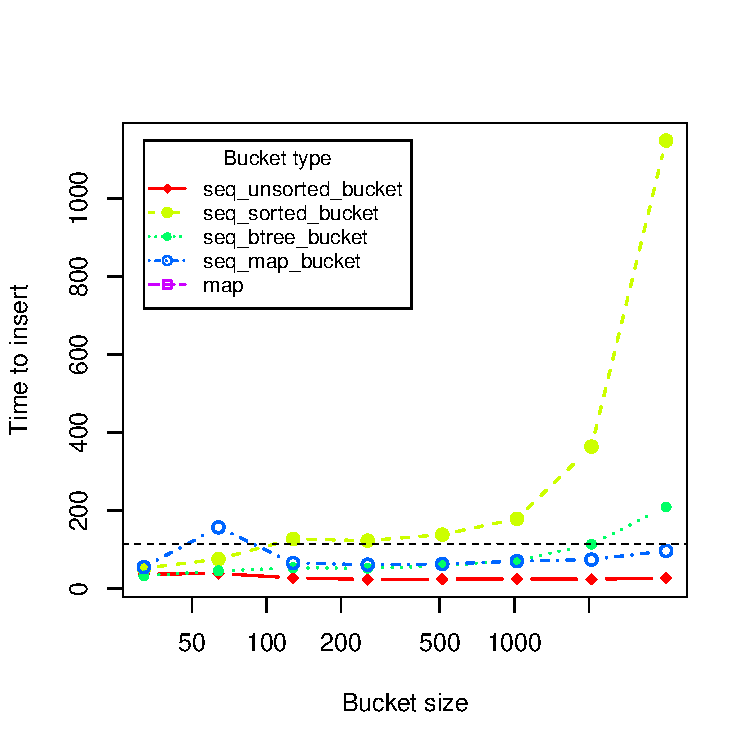
\includegraphics[width=1.0\textwidth]{plots/i7_30m_insert}
        }
        \subfloat[Search]{
            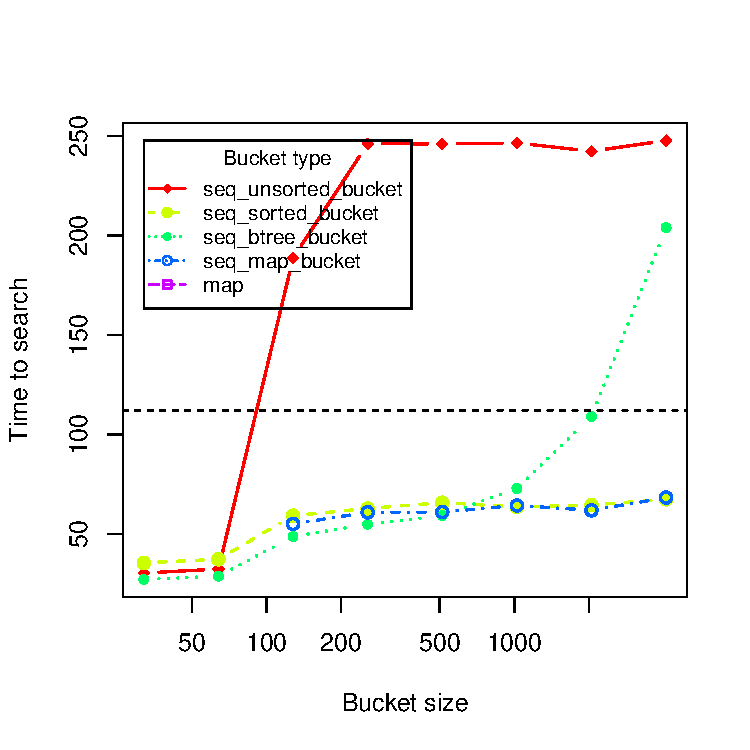
\includegraphics[width=1.0\textwidth]{plots/i7_30m_search}
        }
        \caption{Scaling of insertion and self-search times using the 30M Random
        dataset, with varying bucket sizes from 32 to 4096. The {\keyword map} time
        is shown for reference as a dotted line.}
        \label{fig:seq_30m}
    \end{figure*}
\end{landscape}



\section{Parallel scaling}
In testing the parallel scaling of the different burst trie variants,
a  

Locking improvement: per-node lock.

Amdahls law.


\subsection{Datasets}


These tests show a clear bottleneck already beginning to show at 2 cores for
insertions, while the concurrent locking on insertions allows full parallelism
to the order of the number of cores available. This is caused by the shallow
trie, which is an issue due to node-level parallelism.

Due to sharing of the locks, that needs to be synchronized between caches, on
an expensive interconnect, the scaling is negative. That is, the overhead
created by synchronization of the node locks is greater than the gain in
parallelism.

\begin{table}[h]
    \centering
    \begin{tabular}[here]{ l l l l }
    \hline
        Bucket type            & Size & Insert & Search\\\hline
        %
        STL::Map               & 256  & 1.768  & 5.441\\
        Sorted dynamic array   & 256  & 3.301  & 5.261\\
        Unsorted dynamic array & 64   & 1.030  & 3.644\\
        Unsorted dynamic array & 128+ & ~0.600 & 6.108\\
        Binary tree            & 128  & 1.523  & 4.938\\
        Binary tree            & 32   & 0.979  & 5.680\\
    \hline
    \end{tabular}
    \caption{Speedup factor for each bucket in the 30M dataset for 32 threads on the i7
quad-core machine (virtual octo-core).}
    \label{tab:speedups_30m_i7}
\end{table}

This shows that it is possible to obtain speedup factors of up to 6 with a
fully concurrent locking mechanism. With this as the reference, the gains
of a factor $3.3$ on insertions and a factor $5.2$ on searches, the sorted
dynamic arrays seem to scale the best.

The greatest gains appearing from unsorted array concurrency is evidence that
the locking favors heavy work the leaves. This fits perfectly with the expected
node-level parallelism, which also explains why the greatest gains in insertion
is seen with sorted arrays, being the only bucket structure with linear insertion
times, and thereby up to $O(n^2)$ bursting times.

It is somewhat surprising that the searches take such a big hit from the locking,
evident in the larger unsorted array cases. The empirical concurrency of the
read-locks is hereby reduced. The difference is even greater on the Xeon machine,
where the maximum speedup factor observed for searching was 4.1.
